\chapter{Teoría de números}

\index{teoría de números}

La \key{teoría de números} es una rama de las matemáticas
que estudia los enteros.
La teoría de números es un campo fascinante,
porque muchas preguntas que involucran enteros
son muy difíciles de resolver incluso si parecen
simples a primera vista. Por ejemplo, considera la
siguiente ecuación:
\[x^3 + y^3 + z^3 = 33\]
Es fácil encontrar tres números reales $x$, $y$, y $z$
que satisfagan la ecuación.
Por ejemplo, podemos elegir
\[
    \begin{array}{lcl}
        x = 3,           \\
        y = \sqrt[3]{3}, \\
        z = \sqrt[3]{3}. \\
    \end{array}
\]
Sin embargo, es un problema abierto en teoría de números
si hay tres
\emph{enteros} $x$, $y$, y $z$
que satisfagan la ecuación \cite{bec07}.

En este capítulo, nos centraremos en conceptos básicos
y algoritmos en teoría de números.
A lo largo del capítulo, asumiremos que todos los números
son enteros si no se indica lo contrario.

\section{Primos y factores}

\index{divisibilidad}
\index{factor}
\index{divisor}

Un número $a$ se llama \key{factor} o \key{divisor} de un número $b$
si $a$ divide a $b$.
Si $a$ es un factor de $b$,
escribimos $a \mid b$, y de lo contrario escribimos $a \nmid b$.
Por ejemplo, los factores de 24 son
1, 2, 3, 4, 6, 8, 12 y 24.

\index{primo}
\index{descomposición en primos}
\index{factorización en primos}

Un número $n>1$ es \key{primo}
si sus únicos factores positivos son 1 y $n$.
Por ejemplo, 7, 19 y 41 son primos,
pero 35 no es un primo, porque $5 \cdot 7 = 35$.
Para cada número $n>1$, existe una única
\key{descomposición en factores primos}
\[ n = p_1^{\alpha_1} p_2^{\alpha_2} \cdots p_k^{\alpha_k},\]
donde $p_1,p_2,\ldots,p_k$ son primos distintos y
$\alpha_1,\alpha_2,\ldots,\alpha_k$ son números positivos.
Por ejemplo, la descomposición en factores primos de 84 es
\[84 = 2^2 \cdot 3^1 \cdot 7^1.\]

El \key{número de factores} de un número $n$ es
\[\tau(n)=\prod_{i=1}^k (\alpha_i+1),\]
porque para cada primo $p_i$, hay
$\alpha_i+1$ formas de elegir cuántas veces
aparece en el factor.
Por ejemplo, el número de factores
de 84 es
$\tau(84)=3 \cdot 2 \cdot 2 = 12$.
Los factores son
1, 2, 3, 4, 6, 7, 12, 14, 21, 28, 42 y 84.

La \key{suma de factores} de $n$ es
\[\sigma(n)=\prod_{i=1}^k (1+p_i+\ldots+p_i^{\alpha_i}) = \prod_{i=1}^k \frac{p_i^{a_i+1}-1}{p_i-1},\]
donde la última fórmula se basa en la fórmula de progresión geométrica.
Por ejemplo, la suma de factores de 84 es
\[\sigma(84)=\frac{2^3-1}{2-1} \cdot \frac{3^2-1}{3-1} \cdot \frac{7^2-1}{7-1} = 7 \cdot 4 \cdot 8 = 224.\]

El \key{producto de factores} de $n$ es
\[\mu(n)=n^{\tau(n)/2},\]
porque podemos formar $\tau(n)/2$ pares a partir de los factores,
cada uno con producto $n$.
Por ejemplo, los factores de 84
producen los pares
$1 \cdot 84$, $2 \cdot 42$, $3 \cdot 28$, etc.,
y el producto de los factores es $\mu(84)=84^6=351298031616$.

\index{número perfecto}

Un número $n$ se llama \key{número perfecto} si $n=\sigma(n)-n$,
es decir, $n$ es igual a la suma de sus factores
entre $1$ y $n-1$.
Por ejemplo, 28 es un número perfecto,
porque $28=1+2+4+7+14$.

\subsubsection{Número de primos}

Es fácil demostrar que hay una cantidad infinita
de números primos.
Si el número de primos fuera finito,
podríamos construir un conjunto $P=\{p_1,p_2,\ldots,p_n\}$
que contuviera todos los primos.
Por ejemplo, $p_1=2$, $p_2=3$, $p_3=5$, y así sucesivamente.
Sin embargo, usando $P$, podríamos formar un nuevo primo
\[p_1 p_2 \cdots p_n+1\]
que es más grande que todos los elementos en $P$.
Esta es una contradicción, y el número de primos
tiene que ser infinito.

\subsubsection{Densidad de primos}

La densidad de primos significa cuán a menudo hay primos
entre los números.
Decimos que $\pi(n)$ denota el número de primos entre
$1$ y $n$. Por ejemplo, $\pi(10)=4$, porque
hay 4 primos entre $1$ y $10$: 2, 3, 5 y 7.

Es posible demostrar que
\[\pi(n) \approx \frac{n}{\ln n},\]
lo que significa que los primos son bastante frecuentes.
Por ejemplo, el número de primos entre
$1$ y $10^6$ es $\pi(10^6)=78498$,
y $10^6 / \ln 10^6 \approx 72382$.

\subsubsection{Conjeturas}

Hay muchas \emph{conjeturas} relacionadas con los números primos.
La mayoría de las personas piensan que las conjeturas son verdaderas,
pero nadie ha podido demostrarlas todavía. Algunos ejemplos de conjeturas
famosas son:

\begin{itemize}
    \index{Conjetura de Goldbach}
    \item \key{Conjetura de Goldbach}:
          Cada número entero par $n>2$ puede representarse como una
          suma de dos números primos.
          \index{números primos gemelos}
    \item \key{Conjetura de los primos gemelos}:
          Hay una cantidad infinita de pares
          de la forma $\{p,p+2\}$,
          donde tanto $p$ como $p+2$ son primos.
          \index{Conjetura de Legendre}
    \item \key{Conjetura de Legendre}:
          Siempre hay un número primo entre los números
          $n^2$ y $(n+1)^2$, donde $n$ es cualquier número entero positivo.
\end{itemize}

\subsubsection{Algoritmos básicos}

Si un número $n$ no es primo,
se puede representar como un producto $a \cdot b$,
donde $a \le \sqrt n$ o $b \le \sqrt n$,
por lo que ciertamente tiene un factor entre $2$ y $\lfloor \sqrt n \rfloor$.
Usando esta observación, podemos probar
si un número es primo y encontrar la factorización en primos
de un número en tiempo $O(\sqrt n)$.

La siguiente función \texttt{esPrimo} verifica
si el número dado $n$ es primo.
La función intenta dividir $n$ por
cada número entre $2$ y $\lfloor \sqrt n \rfloor$,
y si ninguno de ellos divide a $n$, entonces $n$ es primo.

\begin{lstlisting}
bool esPrimo(int n) {
    if (n < 2) return false;
    for (int x = 2; x * x <= n; x++) {
        if (n % x == 0) return false;
    }
    return true;
}
\end{lstlisting}

\noindent
La siguiente función \texttt{factores}
construye un vector que contiene la factorización
prima de $n$.
La función divide $n$ por sus factores primos,
y los agrega al vector.
El proceso termina cuando el número restante $n$
no tiene factores entre $2$ y $\lfloor \sqrt n \rfloor$.
Si $n>1$, es primo y el último factor.

\begin{lstlisting}
vector<int> factores(int n) {
    vector<int> f;
    for (int x = 2; x * x <= n; x++) {
        while (n % x == 0) {
            f.push_back(x);
            n /= x;
        }
    }
    if (n > 1) f.push_back(n);
    return f;
}
\end{lstlisting}

Ten en cuenta que cada factor primo aparece en el vector
tantas veces como divide el número.
Por ejemplo, $24=2^3 \cdot 3$,
así que la función devuelve $[2,2,2,3]$.

\subsubsection{Criba de Eratóstenes}

\index{criba de Eratóstenes}

La \key{criba de Eratóstenes}
es un algoritmo de preprocesamiento
que construye una matriz con la que podemos
comprobar de manera eficiente si un número dado entre $2 \ldots n$
es primo y, si no lo es, encontrar un factor primo del número.

El algoritmo construye una matriz $\texttt{criba}$
cuyas posiciones $2,3,\ldots,n$ se utilizan.
El valor $\texttt{criba}[k]=0$ significa
que $k$ es primo,
y el valor $\texttt{criba}[k] \neq 0$
significa que $k$ no es un primo y uno
de sus factores primos es $\texttt{criba}[k]$.

El algoritmo itera a través de los números
$2 \ldots n$ uno por uno.
Siempre que se encuentra un nuevo primo $x$,
el algoritmo registra que los múltiplos
de $x$ ($2x,3x,4x,\ldots$) no son primos,
porque el número $x$ los divide.

Por ejemplo, si $n=20$, la matriz es la siguiente:

\begin{center}
    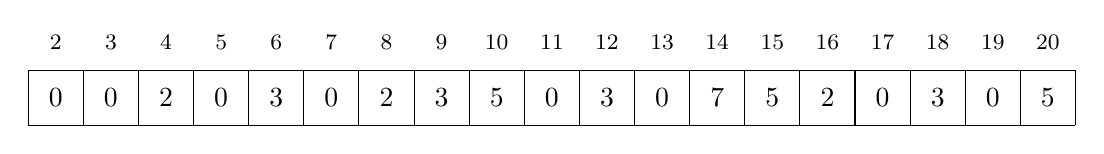
\begin{tikzpicture}[scale=0.7]
        \draw (0,0) grid (19,1);

        \node at (0.5,0.5) {$0$};
        \node at (1.5,0.5) {$0$};
        \node at (2.5,0.5) {$2$};
        \node at (3.5,0.5) {$0$};
        \node at (4.5,0.5) {$3$};
        \node at (5.5,0.5) {$0$};
        \node at (6.5,0.5) {$2$};
        \node at (7.5,0.5) {$3$};
        \node at (8.5,0.5) {$5$};
        \node at (9.5,0.5) {$0$};
        \node at (10.5,0.5) {$3$};
        \node at (11.5,0.5) {$0$};
        \node at (12.5,0.5) {$7$};
        \node at (13.5,0.5) {$5$};
        \node at (14.5,0.5) {$2$};
        \node at (15.5,0.5) {$0$};
        \node at (16.5,0.5) {$3$};
        \node at (17.5,0.5) {$0$};
        \node at (18.5,0.5) {$5$};

        \footnotesize

        \node at (0.5,1.5) {$2$};
        \node at (1.5,1.5) {$3$};
        \node at (2.5,1.5) {$4$};
        \node at (3.5,1.5) {$5$};
        \node at (4.5,1.5) {$6$};
        \node at (5.5,1.5) {$7$};
        \node at (6.5,1.5) {$8$};
        \node at (7.5,1.5) {$9$};
        \node at (8.5,1.5) {$10$};
        \node at (9.5,1.5) {$11$};
        \node at (10.5,1.5) {$12$};
        \node at (11.5,1.5) {$13$};
        \node at (12.5,1.5) {$14$};
        \node at (13.5,1.5) {$15$};
        \node at (14.5,1.5) {$16$};
        \node at (15.5,1.5) {$17$};
        \node at (16.5,1.5) {$18$};
        \node at (17.5,1.5) {$19$};
        \node at (18.5,1.5) {$20$};

    \end{tikzpicture}
\end{center}

El siguiente código implementa la criba de
Eratóstenes.
El código asume que cada elemento de
\texttt{criba} es inicialmente cero.

\begin{lstlisting}
for (int x = 2; x <= n; x++) {
    if (criba[x]) continue;
    for (int u = 2*x; u <= n; u += x) {
        criba[u] = x;
    }
}
\end{lstlisting}

El bucle interno del algoritmo se ejecuta
$n/x$ veces para cada valor de $x$, por lo que
un límite superior para el tiempo de ejecución
del algoritmo es la suma armónica
\[\sum_{x=2}^n n/x = n/2 + n/3 + n/4 + \cdots + n/n = O(n \log n).\]

\index{suma armónica}

De hecho, el algoritmo es más eficiente,
porque el bucle interno solo se ejecutará si
el número $x$ es primo.
Se puede demostrar que el tiempo de ejecución del
algoritmo es solo $O(n \log \log n)$,
una complejidad muy cercana a $O(n)$.

\subsubsection{Algoritmo de Euclides}

\index{máximo común divisor}
\index{mínimo común múltiplo}
\index{algoritmo de Euclides}

El \key{máximo común divisor} de
números $a$ y $b$, $\textrm{mcd}(a,b)$,
es el número más grande que divide tanto a $a$ como a $b$,
y el \key{mínimo común múltiplo} de
$a$ y $b$, $\textrm{mcm}(a,b)$,
es el número más pequeño que es divisible por
ambos $a$ y $b$.
Por ejemplo,
$\textrm{mcd}(24,36)=12$ y
$\textrm{mcm}(24,36)=72$.

El máximo común divisor y el mínimo común múltiplo
están conectados de la siguiente manera:
\[\textrm{mcm}(a,b)=\frac{ab}{\textrm{mcd}(a,b)}\]

El \key{algoritmo de Euclides}\footnote{Euclides fue un matemático griego que
    vivió alrededor del año 300 a.C. Este es quizás el primer algoritmo conocido en la historia.} proporciona una forma eficiente
para encontrar el máximo común divisor de dos números.
El algoritmo se basa en la siguiente fórmula:
\begin{equation*}
    \textrm{mcd}(a,b) = \begin{cases}
        a                         & b = 0    \\
        \textrm{mcd}(b,a \bmod b) & b \neq 0 \\
    \end{cases}
\end{equation*}

Por ejemplo,
\[\textrm{mcd}(24,36) = \textrm{mcd}(36,24)= \textrm{mcd}(24,12) = \textrm{mcd}(12,0)=12.\]

El algoritmo se puede implementar de la siguiente manera:
\begin{lstlisting}
int mcd(int a, int b) {
    if (b == 0) return a;
    return mcd(b, a%b);
}
\end{lstlisting}

Se puede demostrar que el algoritmo de Euclides funciona
en tiempo $O(\log n)$, donde $n=\min(a,b)$.
El peor caso para el algoritmo es
cuando $a$ y $b$ son números consecutivos de Fibonacci.
Por ejemplo,
\[\textrm{mcd}(13,8)=\textrm{mcd}(8,5)
    =\textrm{mcd}(5,3)=\textrm{mcd}(3,2)=\textrm{mcd}(2,1)=\textrm{mcd}(1,0)=1.\]

\subsubsection{Función $\varphi$ de Euler}

\index{coprimo}
\index{Función $\varphi$ de Euler}

Los números $a$ y $b$ son \key{coprimos}
si $\textrm{mcd}(a,b)=1$.
La \key{función $\varphi$ de Euler} $\varphi(n)$
%\footnote{Euler presentó esta función en 1763.}
da la cantidad de números coprimos a $n$
entre $1$ y $n$.
Por ejemplo, $\varphi(12)=4$,
porque 1, 5, 7 y 11
son coprimos a 12.

El valor de $\varphi(n)$ se puede calcular
a partir de la factorización en primos de $n$
usando la fórmula
\[ \varphi(n) = \prod_{i=1}^k p_i^{\alpha_i-1}(p_i-1). \]
Por ejemplo, $\varphi(12)=2^1 \cdot (2-1) \cdot 3^0 \cdot (3-1)=4$.
Nota que $\varphi(n)=n-1$ si $n$ es primo.

\section{Aritmética modular}

\index{aritmética modular}

En la \key{aritmética modular},
el conjunto de números está limitado de tal manera que
solo se utilizan los números $0,1,2,\ldots,m-1$,
donde $m$ es una constante.
Cada número $x$ es
representado por el número $x \bmod m$:
el resto luego de dividir $x$ por $m$.
Por ejemplo, si $m=17$, entonces $75$
es representado por $75 \bmod 17 = 7$.

A menudo podemos tomar residuos antes de realizar
cálculos.
En particular, se cumplen las siguientes fórmulas:
\[
    \begin{array}{rcl}
        (x+y) \bmod m       & = & (x \bmod m + y \bmod m) \bmod m     \\
        (x-y) \bmod m       & = & (x \bmod m - y \bmod m) \bmod m     \\
        (x \cdot y) \bmod m & = & (x \bmod m \cdot y \bmod m) \bmod m \\
        x^n \bmod m         & = & (x \bmod m)^n \bmod m               \\
    \end{array}
\]

\subsubsection{Exponenciación modular}

A menudo es necesario calcular el valor de $x^n \bmod m$ eficientemente.
Esto puede hacerse en $O(\log n)$ utilizando la siguiente recursión:
\begin{equation*}
    x^n = \begin{cases}
        1                     & n = 0               \\
        x^{n/2} \cdot x^{n/2} & \text{$n$ es par}   \\
        x^{n-1} \cdot x       & \text{$n$ es impar}
    \end{cases}
\end{equation*}

Es importante que en el caso de un $n$ impar, el valor de $x^{n/2}$ solo
se compute una vez. Esto garantiza que la complejidad temporal del algoritmo
sea $O(\log n)$, porque $n$ siempre se divide en dos cuando es par.

La siguiente función calcula el valor de $x^n \bmod m$:

\begin{lstlisting}
int exp_mod(int x, int n, int m) {
    if (n == 0) return 1 % m;
    long long u = exp_mod(x, n / 2, m);
    u = (u * u) % m;
    if (n % 2 == 1) u = (u * x) % m;
    return u;
}
\end{lstlisting}

\subsubsection{Teorema de Fermat y teorema de Euler}

\index{teorema de Fermat}
\index{teorema de Euler}

El \key{teorema de Fermat} dice que
\[x^{m-1} \bmod m = 1\]
cuando $m$ es primo y $x$ y $m$ son coprimos. Esto también resulta en
\[x^k \bmod m = x^{k \bmod (m-1)} \bmod m.\]
Más generalmente, el \key{teorema de Euler} establece que
\[x^{\varphi(m)} \bmod m = 1\]
cuando $x$ y $m$ son coprimos. El teorema de Fermat sigue del teorema
de Euler, porque si $m$ es primo, entonces $\varphi(m)=m-1$.

\subsubsection{Inverso modular}

\index{inverso modular}

El inverso de $x$ módulo $m$ es un número $x^{-1}$ tal que
\[ x x^{-1} \bmod m = 1. \]
Por ejemplo, si $x=6$ y $m=17$, entonces $x^{-1}=3$, porque
$6\cdot3 \bmod 17=1$.

Utilizando inversos modulares, podemos dividir números módulo $m$, porque
la división por $x$ corresponde a la multiplicación por $x^{-1}$. Por ejemplo,
para evaluar el valor de $36/6 \bmod 17$, podemos usar la fórmula
$2 \cdot 3 \bmod 17$, porque $36 \bmod 17 = 2$ y $6^{-1} \bmod 17 = 3$.

De todas formas, un inverso modular no siempre existe. Por ejemplo, si $x=2$
y $m=4$, la ecuación
\[ x x^{-1} \bmod m = 1 \]
no puede resolverse, porque todos los múltiplos de 2 son pares y el resto
nunca puede ser 1 cuando $m=4$. Resulta que el valor de $x^{-1} \bmod m$
puede ser calculado exactamente cuando $x$ y $m$ son coprimos.

Si existe un inverso modular, puede ser calculado utilizando la fórmula
\[
    x^{-1} = x^{\varphi(m)-1}.
\]
Si $m$ es primo, la fórmula se vuelve
\[
    x^{-1} = x^{m-2}.
\]
Por ejemplo,
\[6^{-1} \bmod 17 =6^{17-2} \bmod 17 = 3.\]

Esta fórmula nos permite calcular inversos modulares eficientemente utilizando
el algoritmo de exponenciación modular. Esta fórmula puede ser derivada usando
el algoritmo de Euler. Primero, el inverso modular debe satisfacer la
siguiente ecuación:
\[
    x x^{-1} \bmod m = 1.
\]
Por otro lado, según el teorema de Euler,
\[
    x^{\varphi(m)} \bmod m =  xx^{\varphi(m)-1} \bmod m = 1,
\]
así que los números $x^{-1}$ y $x^{\varphi(m)-1}$ son iguales.

\subsubsection{Aritmética computacional}

En la programación, los enteros sin signo son representados módulo $2^k$,
donde $k$ es el número de bits del tipo de datos. Una consecuencia típica
de esto es que el número ``da la vuelta'' si se vuelve demasiado grande.

Por ejemplo, en C++, los números de tipo \texttt{unsigned int} se representan
módulo $2^{32}$. El siguiente código declara una variable \texttt{unsigned int}
cuyo valor es $123456789$. Luego de esto, el valor se multiplicará por si mismo,
y el resultado es $123456789^2 \bmod 2^{32} = 2537071545$.

\begin{lstlisting}
unsigned int x = 123456789;
cout << x * x << "\n"; // 2537071545
\end{lstlisting}

\section{Resolver ecuaciones}

\subsubsection*{Ecuaciones diofánticas}

\index{ecuacion diofántica}

Una \key{ecuación diofántica} es una ecuación con la forma \[ ax + by = c, \]
donde $a$, $b$, y $c$ son constantes y los valores de $x$ e $y$ deben ser
encontrados. Cada número en la ecuación debe ser un entero. Por ejemplo, una
solución para la ecuación $5x+2y=11$ es $x=3$ y $y=-2$.

\index{algoritmo extendido de Euclides}

Podemos resolver una ecuación diofántica eficientemente utilizando el
algoritmo de Euclides. Resulta que podemos extender el algoritmo de
Euclides tal que encuentre números $x$ e $y$ que satisfagan la siguiente
ecuación: \[ax + by = \textrm{mcd}(a,b)\]

Una ecuación diofántica puede resolverse si $c$ es divisible por
$\textrm{mcd}(a,b)$, y de lo contrario no se puede resolver.

Por ejemplo, encontremos los números $x$ e $y$ que satisfagan la siguiente
ecuación: \[39x + 15y = 12\]

La ecuación se puede resolver, porque $\textrm{mcd}(39,15)=3$ y $3 \mid 12$.
Cuando el algoritmo de Euclides calculo el máximo común divisor de 39 y 15,
produce la siguiente secuencia de llamadas de función:
\[
    \textrm{mcd}(39,15) = \textrm{mcd}(15,9)
    = \textrm{mcd}(9,6) = \textrm{mcd}(6,3)
    = \textrm{mcd}(3,0) = 3 \]
Esto corresponde a las siguientes ecuaciones:
\[
    \begin{array}{lcl}
        39 - 2 \cdot 15 & = & 9 \\
        15 - 1 \cdot 9  & = & 6 \\
        9 - 1 \cdot 6   & = & 3 \\
    \end{array}
\]
Utilizando estas ecuaciones, podemos derivar
\[
    39 \cdot 2 + 15 \cdot (-5) = 3
\]
y multiplicando esto por 4, el resultado es
\[
    39 \cdot 8 + 15 \cdot (-20) = 12,
\]
por lo que una solución a la ecuación es $x=8$ e $y=-20$.

Una solución a una ecuación diofántica no es única, porque podemos formar un
número infinito de soluciones si conocemos una. Si un par $(x,y)$ es una
solución, entonces todos los pares con la siguiente forma, donde $k$ es cualquier entero
\[\left(x+\frac{kb}{\textrm{mcd}(a,b)},y-\frac{ka}{\textrm{mcd}(a,b)}\right)\]
también son soluciones.

\subsubsection{Teorema chino del resto}

\index{teorema chino del resto}

El \key{teorema chino del resto} resuelve un grupo de ecuaciones con la forma
\[
    \begin{array}{lcl}
        x & = & a_1 \bmod m_1 \\
        x & = & a_2 \bmod m_2 \\
        \cdots                \\
        x & = & a_n \bmod m_n \\
    \end{array}
\]
donde todos los pares de $m_1,m_2,\ldots,m_n$ son coprimos.

Definamos $x^{-1}_m$ como el inverso de $x$ módulo $m$, y
\[ X_k = \frac{m_1 m_2 \cdots m_n}{m_k}.\]
Usando esta notación, una solución a la ecuación es
\[x = a_1 X_1 {X_1}^{-1}_{m_1} + a_2 X_2 {X_2}^{-1}_{m_2} + \cdots + a_n X_n {X_n}^{-1}_{m_n}.\]
En esta solución, para cada $k=1,2,\ldots,n$,
\[a_k X_k {X_k}^{-1}_{m_k} \bmod m_k = a_k,\]
porque
\[X_k {X_k}^{-1}_{m_k} \bmod m_k = 1.\]
Dado que todos los otros términos en la suma son divisibles por $m_k$, no
tienen un efecto sobre el resto (módulo), y $x \bmod m_k = a_k$.

Por ejemplo, una solución para
\[
    \begin{array}{lcl}
        x & = & 3 \bmod 5 \\
        x & = & 4 \bmod 7 \\
        x & = & 2 \bmod 3 \\
    \end{array}
\]
es
\[ 3 \cdot 21 \cdot 1 + 4 \cdot 15 \cdot 1 + 2 \cdot 35 \cdot 2 = 263.\]

Una vez que encontramos una solución para $x$, podemos generar una cantidad
infinita de soluciones, porque todos los números con la forma
\[x+m_1 m_2 \cdots m_n\] son soluciones.

\section{Otros resultados}

\subsubsection{Teorema de Lagrange}

\index{teorema de Lagrange}

El \key{teorema de Lagrange} dice que cada entero positivo puede
representarse como una suma de cuatro cuadrados, o sea, $a^2+b^2+c^2+d^2$.
Por ejemplo, el número 123 es representable como la suma $8^2+5^2+5^2+3^2$.

\subsubsection{Teorema de Zeckendorf}

\index{teorema de Zeckendorf}
\index{número de Fibonacci}

El \key{teorema de Zeckendorf} dice que cada entero positivo tiene una
representación única como suma de números de Fibonacci tal que no haya
un par de números iguales o consecutivos en la secuencia de Fibonacci.
Por ejemplo, el número 74 se puede representar como la suma $55+13+5+1$.

\subsubsection{Terna pitagórica}

\index{terna pitagórica}
\index{fórmula de Euclides}

Una \key{terna pitagórica} es un trío de números $(a,b,c)$ que satisfacen
el teorema de Pitágoras $a^2+b^2=c^2$, lo que significa que existe un triángulo
rectángulo con lados $a$, $b$, y $c$. Por ejemplo, $(3,4,5)$ es una terna
pitagórica.

Si $(a,b,c)$ es una terna pitagórica, todas las ternas con la forma $(ka,kb,kc)$
también son ternas pitagóricas donde $k>1$. Una terna pitagórica es
\emph{primitiva} si $a$, $b$, y $c$ son coprimos, y todas las ternas
pitagóricas pueden construirse desde ternas primitivas utilizando un factor $k$.

La \key{fórmula de Euclides} también puede utilizarse para producir todas
las ternas pitagóricas primitivas. Cada de estas tiene la forma
\[(n^2-m^2,2nm,n^2+m^2),\] donde $0<m<n$, $n$ y $m$ son coprimos, y por lo
menos una de $n$ y $m$ es par. Por ejemplo, cuando $m=1$ y $n=2$, la fórmula
produce la mínima terna pitagórica
\[(2^2-1^2,2\cdot2\cdot1,2^2+1^2)=(3,4,5).\]

\subsubsection{Teorema de Wilson}

\index{teorema de Wilson}

El \key{teorema de Wilson} dice que un número $n$ es primo exactamente cuando
\[(n-1)! \bmod n = n-1.\]
Por ejemplo, el número 11 es primo, porque
\[10! \bmod 11 = 10,\]
y el número 12 no es primo, porque
\[11! \bmod 12 = 0 \neq 11.\]

Por lo tanto, el teorema de Wilson puede usarse para revisar si un número
es primero. No obstante, en la práctica el teorema no es aplicable para
grandes valores de $n$, porque es difícil calcular valores de $(n-1)!$
cuando $n$ es grande.
